\section{Compuertas de cómputo cuántico}

Las compuertas cuánticas son el análogo cuántico de las compuertas lógicas utilizadas en cómputo clásico. En un circuito cuántico, las compuertas permiten manipular los qubits. Una compuerta $U$ válida es un operador de evolución unitario que actúa sobre el espacio generado por $n$ qubits (esto es, actúa sobre $\hilbert_{2^{n}}$):
\begin{equation}
  U:\hilbert_{2^{n}}\rightarrow\hilbert_{2^{n}}.\nonumber
\end{equation}
Compuertas de un qubit comunes icluyen a los operadores de Pauli, mientras que para dos qubits existen compuertas como el SWAP, el controlled-not (CNOT), y la compuerta de Hadamard. En este trabajo se analizará la evolución efectiva bajo evoluciones subyacentes descritas por las compuertas SWAP y CNOT. 

\subsection{La compuerta cuántica SWAP}

La compuerta SWAP, $S$, actúa sobre dos qubits permutándolos. \ddnote*{Su acción sobre la base computacional de dos qubits es}{Su acción sobre la base de $\hilbert_{4}$ contruida mediante los eigenestados de $\pauli{3}\otimes\pauli{3}$ es} \ddnote{ojo, no hay una única base de $\pauli{3}\otimes\pauli{3}$, pues el operador es degenerado, es mejor mencionarla base computacional, y ya}
\begin{align}
    \ket{0}\otimes\ket{0}&\mapsto\ket{0}\otimes\ket{0}\nonumber\\
    \ket{0}\otimes\ket{1}&\mapsto\ket{1}\otimes\ket{0}\nonumber\\
    \ket{1}\otimes\ket{0}&\mapsto\ket{0}\otimes\ket{1}\nonumber\\
    \ket{1}\otimes\ket{1}&\mapsto\ket{1}\otimes\ket{0} \rlap{.}\nonumber
\end{align}
Si un sistema está descrito por un operador de densidad separable, $\varrho=\rho_{A}\otimes\rho_{B}$, entonces el efecto de la compuerta SWAP es 
\begin{equation}
    S\varrho S=\rho_{B}\otimes\rho_{A}.\nonumber
\end{equation}
\ddnote{El swap es hermítico, quité la dagger}
La compuerta tiene representación como matriz de permutación
\begin{equation}
    S=\begin{pmatrix}
        1&0&0&0\\
        0&0&1&0\\
        0&1&0&0\\
        0&0&0&1
    \end{pmatrix}.\nonumber
\end{equation}
Descrito de esta manera, el operador SWAP es un operador de evolución \textit{discreto}. Esto es, lleva un estado $\varrho$ a otro $\varrho'$ sin considerar ninguna dependencia temporal ni ningún estado intermedio. Sin embargo, como esta evolución es unitaria, es extendible a cualquier tiempo dado el hamiltoniano adecuado. Consideramos entonces
\begin{equation}
  H_{S}=\omega\sum_{i=1}^{3}\pauli{i}\otimes\pauli{i}\nonumber
\end{equation}
que, tomando $\omega=\frac{\pi}{4}$, genera una compuerta SWAP al tiempo $t=1$. Dado este hamiltoniano, la forma matricial del operador \textsc{SWAP} a un tiempo $t$ es
\begin{equation}\label{eq:SWAP(t)}
S^{t}=\begin{pmatrix}
 1 & 0 & 0 & 0 \\
 0 & \frac{1}{2}(1+e^{\rmi \pi t}) & \frac{1}{2} (1-e^{\rmi \pi t}) & 0 \\
 0 & \frac{1}{2}(1-e^{\rmi \pi t}) & \frac{1}{2}(1+e^{\rmi \pi t}) & 0 \\
 0 & 0 & 0 & 1
\end{pmatrix}=\begin{pmatrix}
  1 & 0 & 0 & 0 \\
  0 & e^{\rmi\frac{t\pi}{2}}\cos{\frac{t\pi}{2}} & -\rmi e^{\rmi\frac{t\pi}{2}}\sin{\frac{t\pi}{2}} & 0 \\
  0 & -\rmi e^{i\frac{t\pi}{2}}\sin{\frac{t\pi}{2}} & e^{\rmi\frac{t\pi}{2}}\cos{\frac{t\pi}{2}}  & 0 \\
  0 & 0 & 0 & 1
 \end{pmatrix}
\end{equation}

\subsubsection{Evolución discreta}

Para estudiar la dinámica efectiva de una evolución subyacente descrita por el operador SWAP, primero analizaremos el caso en que no se ha introducido la dependencia temporal. Sea $\rho_{\ef}\in\densityspace{2}$ el estado efectivo y $\varrho_{\max}\in\densityspace{4}$ el estado de máxima entropía compatible con $\rho_{\ef}$ y la aplicación de grano grueso descrita en la sección \ref{sec:CH2CG} según $\mcA_{\mcC}^{\max}(\rho_{\ef})=\varrho_{\max}$. Estudiaremos la asignación
\begin{equation}
  \rho_{\ef}\mapsto \mcC(S \varrho_{\max} S).
\end{equation}
\ddnote{quité dagger}
Como el estado de máxima entropía es separable, la acción del operador SWAP sobre este es
\begin{equation}
  \frac{e^{p_{1}\sum_{i}\lambda_{i}\sigma_{i}}}{Z_{1}} \otimes \frac{e^{p_{2}\sum_{i}\lambda_{i}\sigma_{i}}}{Z_{2}}\mapsto\frac{e^{p_{2}\sum_{i}\lambda_{i}\sigma_{i}}}{Z_{2}}\otimes\frac{e^{p_{1}\sum_{i}\lambda_{i}\sigma_{i}}}{Z_{1}}.\nonumber
\end{equation}
El estado de la izquierda corresponde a $\varrho_{\max}(t=0)$, mientras que el de la derecha corresponde a $\varrho_{\max}(t=1)$. Con esto, basta con aplicar la aplicación de grano grueso a ambos estados para hallar a los estados efectivos inicial y final en términos de los multiplicadores de Lagrange:
\begin{equation}
\rho_{\ef}=\frac{1}{2}[\Id+(\hat{r}_{\ef}\cdot\vec{\sigma})(p_{1}\tanh{\lambda p_{1}}+p_{2}\tanh{\lambda p_{2}})],
\end{equation}
\begin{equation}
\Gamma_{t=1}(\rho_{\ef})=\frac{1}{2}[\Id+(\hat{r}_{\ef}\cdot\vec{\sigma})(p_{2}\tanh{\lambda p_{1}}+p_{1}\tanh{\lambda p_{2}})].
\end{equation}
Vemos que ambos estados tienen la misma orientación (orientación significando la dirección del vector de Bloch) pero pureza distinta. Esto significa que el efecto del \textsc{SWAP} subyacente sobre la esfera de Bloch es comprimir al estado efectivo inicial con un coeficiente $\kappa_{1}$ definido según
\begin{equation}\label{eq:SWAPFactor}
  \kappa_{1}=\frac{r_{\ef}(0)}{r_{\ef}(1)}=\frac{p_{2}\tanh{\lambda p_{1}}+p_{1}\tanh{\lambda p_{2}}}{
    p_{1}\tanh{\lambda p_{1}}+p_{2}\tanh{\lambda p_{2}}}.
\end{equation}
Claro está, el factor de compresión depende del multiplicador de Lagrange, que a su vez es una función de la pureza del estado inicial. La figura \ref{fig:SWAPFactor2Drl} muestra dicha dependencia. Como la dependencia en el estado inicial incluye únicamente la pureza del mismo, por lo que la compresión no depende de la dirección. Esta dinámica no es si no un canal de despolarización no lineal. Si la dependencia del factor de despolarización en el estado efectivo inicial se denota por un superíndice, la dinámica efectiva puede escribirse como
\begin{equation}\label{eq:EffectiveSWAP1}
  \Gamma_{t=1}(\rho_{\ef})=\kappa_{1}^{\rho_{\ef}}\rho_{\ef}+(1-\kappa_{1}^{\rho_{\ef}})\frac{1}{2}\Id
\end{equation}
\begin{figure}[ht!]
  \centering
  \begin{subfigure}{0.5\textwidth}
    \centering
    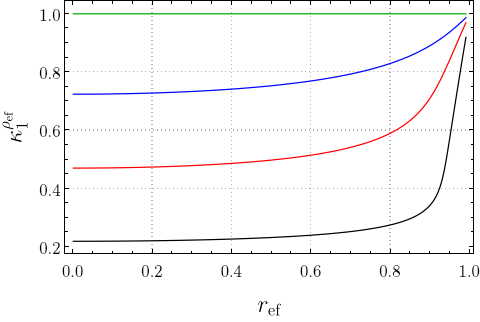
\includegraphics[width=0.9\linewidth]{chapter3/figures_toy/K(r).png}
  \end{subfigure}%
  \begin{subfigure}{0.5\textwidth}
    \centering
    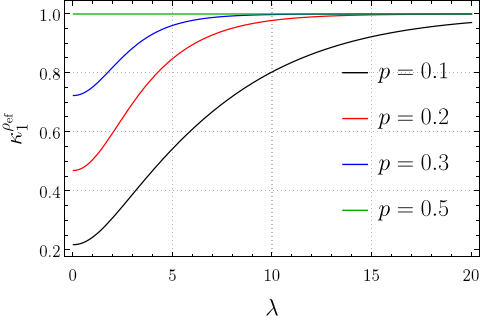
\includegraphics[width=0.9\linewidth]{chapter3/figures_toy/K(lambda).png}
  \end{subfigure}
  \caption{Factor de despolarización $\kappa_{1}^{\rho_{\ef}}$ como función de $r_{\ef}$ (der.) y como función de $\lambda$ (izq.), para diferentes valores de $p_{1}$.}\label{fig:SWAPFactor2Drl}
\end{figure}


De las ecuaciones (\ref{eq:SWAPFactor}) y (\ref{eq:EffectiveSWAP1}) distinguimos lo siguiente:
\begin{itemize}
  \item Si $p_{1}=\frac{1}{2}$, entonces $\kappa_{1}^{\rho_{\ef}}=1$. Esto se debe a que la aplicación borrosa es invariante bajo el $\textsc{SWAP}$ si $p_{1}=\frac{1}{2}$. Así, todos los estado gruesos son puntos fijos bajo una evolución subyacente SWAP con aplicación de grano grueso con parámetro $p_{1}=\frac{1}{2}$.
  \item $\kappa_{1}^{\rho_{\ef}}$ no depende de la orientación del vector de Bloch, únicamente depende de la magnitud $r_{\ef}(0)$ y $p_{1}$.
  \item En los casos extremos, $p_{1}=1$ o $p_{1}=0$, la esfera colapsa al origen.
\end{itemize}


Como el factor de despolarización depende de $\lambda$, la dinámica no es lineal. Las operaciones cuánticas de un qubit se traducen como aplicaciones afines en la esfera de Bloch. Si quisiéramos ver el proceso asociado al \textsc{SWAP} subyacente como una transformación de la forma
\begin{equation}
  \vec{r}\rightarrow M\vec{r}+\vec{c}\nonumber
\end{equation}
en la que $\vec{c}=0$, y $M=OS$ con $O=\Id$ y $S=\kappa_{1}^{\rho_{\ef}}=\Id$, de tal forma que
\begin{equation}
  \vec{r}\rightarrow \kappa_{1}^{\rho_{\ef}}=\vec{r}\nonumber
\end{equation}
\ddnote{error en ecuación, supongo que el $=$ no va.}
nos daríamos cuenta que la transformación no es afín, y por esto, el proceso no puede ser descrito a través del formalismo de las operaciones cuánticas (no tiene representación en operadores de Kraus) \cite{Chuang}.

\subsubsection{Evolución continua}

Utilizando la forma dependiente del tiempo del operador $S$ dada por la ecuación (\ref{eq:SWAP(t)}), puede seguirse el mismo proceso para hallar una expresión del estado efectivo evolucionado como función del tiempo y en términos de los operadores de Lagrange:
\begin{align}
  \begin{split}
  \Gamma_{t}(\rho_{\ef})=\frac{1}{2}\{\Id+(\hat{r_{\ef}}\cdot\vec{\sigma})[&(p_{2}\cos^{2}{\frac{\pi t}{2}}+p_{1}\sin^{2}{\frac{\pi t}{2}})\tanh{p_{1}\lambda}\\
  &+(p_{1}\cos^{2}{\frac{\pi t}{2}}+p_{2}\sin^{2}{\frac{\pi t}{2}})\tanh{p_{2}\lambda}]\}.
  \end{split}
\end{align}
\ddnote{arreglar llaves}
El estado efectivo inicial siendo el mismo, el estado final vuelve a tener la misma orientación, y entonces es posible calcular el factor de despolarización como la razón entre las normas de los vectores de Bloch de los estados inicial y final:
\begin{equation}\label{eq:SWAPFactort}
  \kappa_{t}^{\rho_{\ef}}=\frac{(p_{2}\cos^{2}{\frac{\pi t}{2}}+p\sin^{2}{\frac{\pi t}{2}})\tanh{\lambda p_{1}}+(p_{1}\cos^{2}{\frac{\pi t}{2}}+p_{2}\sin^{2}{\frac{\pi t}{2}})\tanh{\lambda p_{2}}}{
    p_{1}\tanh{\lambda p_{1}}+p_{2}\tanh{\lambda p_{2}}}
\end{equation}

Nuevamente, el factor de despolarización (y por consiguiente, toda la evolución) depende de la pureza del estado efectivo incial, codificada en los multiplicadores de Lagrange. El efecto gradual de la evolución sobre la esfera de Bloch puede verse en la figura \ref{fig:SWAPFactorSequence}. La dinámica efectiva puede escribirse como
\begin{equation}\label{eq:EffectiveSWAPt}
  \boxed{\Gamma_{t}(\rho_{\ef})=\kappa_{t}^{\rho_{\ef}}\rho_{\ef}+(1-\kappa_{t}^{\rho_{\ef}})\frac{1}{2}\Id}
\end{equation}

\begin{figure}[ht!]
  \centering
  \begin{subfigure}{0.32\textwidth}
    \centering
    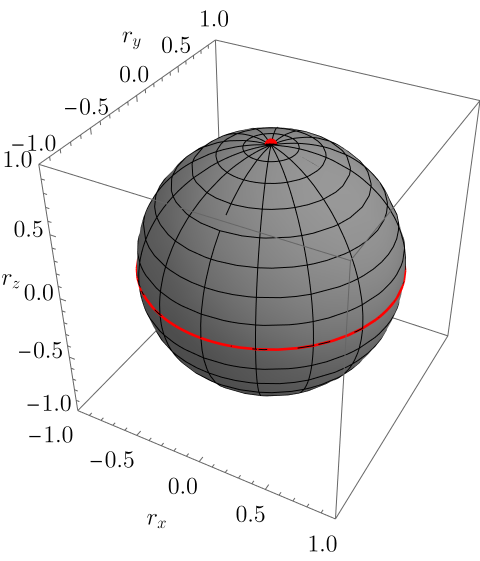
\includegraphics[width=0.9\linewidth]{chapter3/figures_toy/SWAP_t=0._p=0.9_r=0.9.png}
    \caption{$t=0$}
  \end{subfigure}%
  \begin{subfigure}{0.32\textwidth}
    \centering
    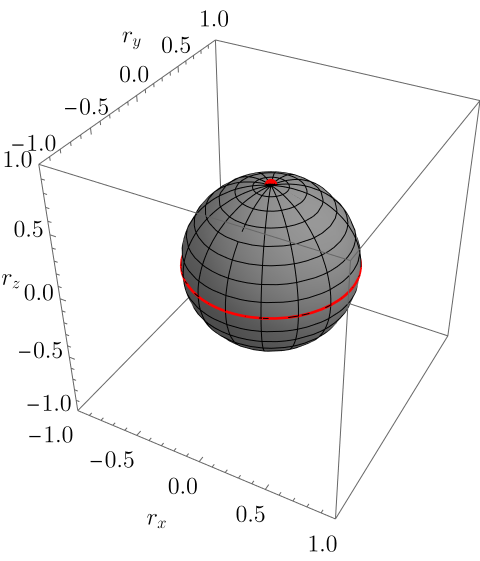
\includegraphics[width=0.9\linewidth]{chapter3/figures_toy/SWAP_t=0.5_p=0.9_r=0.9.png}
    \caption{$t=0.5$}
  \end{subfigure}
  \begin{subfigure}{0.32\textwidth}
    \centering
    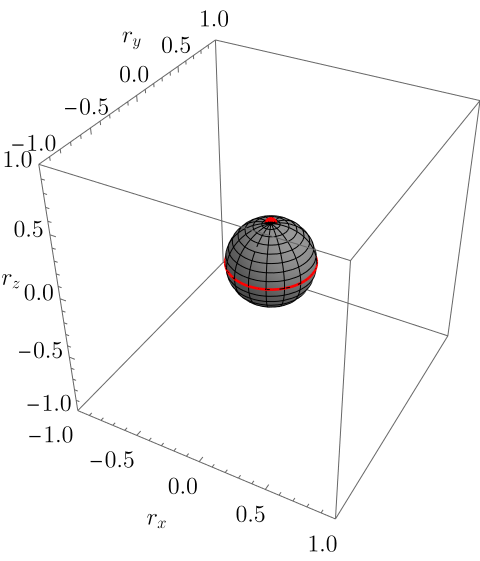
\includegraphics[width=0.9\linewidth]{chapter3/figures_toy/SWAP_t=1._p=0.9_r=0.9.png}
    \caption{$t=1$}
  \end{subfigure}
  \caption{Efecto de la evolución subyacente si $r_{\ef}(0)=0.9$, $p_{1}=0.9$. La dramática contracción se asocia a una pérdida casi total de información. \ddnote{autocontenido}}
  \label{fig:SWAPFactorSequence}
  \end{figure}

De las ecuaciones (\ref{eq:SWAPFactort}) y (\ref{eq:EffectiveSWAPt}) es posible concluir:
\begin{itemize}
  \item $\kappa_{t}^{\rho_{\ef}}$ es una función periódica del tiempo, y su periodo es de $T=2$ (observable en la figura \ref{fig:SWAPFactor2Dt}). Esto viene de que el operador SWAP, además de ser unitario, es hermitiano, i.e. $SS=\Id$.
  \item $\kappa_{t}^{\rho_{\ef}}$ es una función decreciente en $0\leq t\leq 1$.
  \item Se cumplen las observaciones hechas para el caso discreto: la esfera colapsa al origen si $p_{1}=1$ o $p_{1}=0$, y los puntos se mantienen fijos si $p_{1}=\frac{1}{2}$.
\end{itemize}

\begin{figure}[ht!]
  \centering
  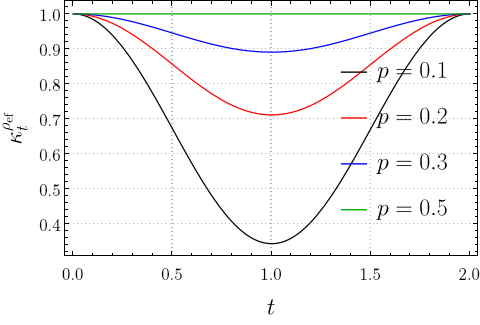
\includegraphics[width=0.6\linewidth]{chapter3/figures_toy/K(t).png}
  \caption{Factor de despolarización $\kappa_{t}^{\rho_{\ef}}$ como función de $t$, para diferentes valores de $p_{1}$ y $r_{\ef}(0)=0.8$.}
  \label{fig:SWAPFactor2Dt}
\end{figure}

En términos del valor esperado del observable $\sigma_{3}$, la evolución del estado se da como
\begin{equation}
  \expval{\sigma_{3}(t)}=\kappa_{t}^{\rho}\expval{\pauli{3}(0)}
\end{equation}
que puede escribirse, también, como las probabilidades de que $\Gamma_{t}(\rho_{\ef})$ se halle en el estado $\ket{0}$ o $\ket{1}$
 \begin{align}
  \bra{0}\Gamma_{t}(\rho_{\ef})\ket{0}=\frac{1}{2}(1+\kappa_{t}^{\rho_{\ef}}\expval{\pauli{3}(0)}) && \bra{1}\Gamma_{t}(\rho_{\ef})\ket{1}=\frac{1}{2}(1-\kappa_{t}^{\rho_{\ef}}\expval{\pauli{3}(0)})
 \end{align}
 donde la dependencia temporal está completamente contenida dentro del factor $\kappa_{t}^{\rho_{\ef}}$. Nótese que el efecto del canal de despolarización es hacer a los estados menos reconocibles entre sí.


\subsection{La compuerta cuántica controlled not}

La compuerta \textit{controlled not}, o CNOT, es el análogo cuántico de la compuerta lógica XOR. La compuerta XOR recibe como entrada dos bits, y arroja uno que puede ser $0$ si los bits de entrada tienen el mismo valor, o $1$ si tienen valores diferentes. Por otro lado, la compuerta cuántica CNOT actúa sobre un sistema de dos qubits, aplicando sobre el segundo qubit la compuerta $\sigma_{1}$ (NOT) si el primer qubit se halla en el estado $\ket{1}$, o dejándolo invariante si el primer qubit se halla en el estado $\ket{0}$. Esto es, cumple que \cite{Chuang}
\begin{align}
    \ket{0}\otimes\ket{0}\mapsto\ket{0}\otimes\ket{0}\nonumber\\
    \ket{0}\otimes\ket{1}\mapsto\ket{0}\otimes\ket{1}\nonumber\\
    \ket{1}\otimes\ket{0}\mapsto\ket{1}\otimes\ket{1}\nonumber\\
    \ket{1}\otimes\ket{1}\mapsto\ket{1}\otimes\ket{0} \rlap{.}\nonumber
\end{align}
\ddnote*{En la base computacional de dos qubits}{En la base de los eigenestados de $\pauli{3}\otimes\pauli{3}$}, la compuerta puede representarse como la matriz de permutación
\begin{equation}
    \cnot=\begin{pmatrix}
        1&0&0&0\\
        0&1&0&0\\
        0&0&0&1\\
        0&0&1&0
    \end{pmatrix}.\nonumber
\end{equation}
Claro está, esta matriz corresponde a la evolución discreta. Considérese el hamiltoniano
\begin{equation}
  H_{\cnot}=-\omega(\pauli{3}\otimes\Id+\Id\otimes\pauli{1}-\pauli{3}\otimes\pauli{1}),\nonumber
\end{equation}
que genera la compuerta CNOT al tiempo $t=1$ cuando $\omega=\frac{\pi}{4}$. Nótese que, por estar conformado por tres operadores que conmutan entre sí, la compuerta puede escribirse como lo acción consecutiva de tres operadores unitarios que conmutan entre sí:
\begin{equation}
  \cnot=(e^{\rmi\omega\pauli{3}}\otimes \Id) (\Id \otimes e^{\rmi\omega\pauli{1}}) e^{-\rmi\omega\pauli{3}\otimes\pauli{1}}.\nonumber
\end{equation}

\subsubsection{CNOT completo efectivo}

Para estudiar la dinámica efectiva del operador $\cnot$ son particularmente útiles las expresiones (\ref{eq:rhoArhoB}). Como el estado de máxima entropía compatible con la aplicación de grano grueso puede escribirse como $\varrho_{\max}=\rho_{1}\otimes\rho_{2}$, entonces hallar el estado efectivo final es un problema de álgebra. En efecto,
\begin{align}
    \Gamma_{t=1}(\rho_{\ef})=&\,\frac{p_{1}}{2}(\rho_{\ef}+\sigma_{3}\rho_{1}\sigma_{3}+\Tr{\sigma_{1}\rho_{2}}[\rho_{1}-\sigma_{3}\rho_{1}\sigma_{3}])\nonumber\\
    &+\frac{p_{2}}{2}(\rho_{\ef}+\sigma_{1}\rho_{2}\sigma_{1}+\Tr{\sigma_{3}\rho_{1}}[\rho_{2}-\sigma_{1}\rho_{2}\sigma_{1}]).\nonumber
\end{align}
La estructura del estado final es una consecuencia directa de la aplicación borrosa. Para entender el significado de cada uno de los términos, considérense dos casos extremos: primero, el caso en que el aparato de medición no tiene un error asociado ($p_{1}=1$). En dicho caso, a través del principio de máxima entropía, se esperaría que el estado efectivo final fuera
\begin{equation}
  \Gamma_{t=1}(\rho_{\ef})=\frac{1}{2}\qty(\rho_{\ef}+\pauli{3}\rho_{\ef}\pauli{3}),\nonumber
\end{equation}
\begin{figure}[ht!]
  \centering
  \begin{subfigure}{0.5\textwidth}
    \centering
    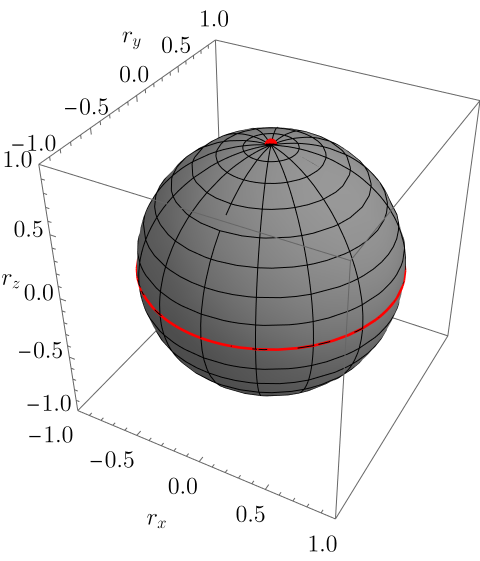
\includegraphics[width=0.6\linewidth]{chapter3/figures_toy/SWAP_t=0._p=0.9_r=0.9.png}
  \end{subfigure}%
  \begin{subfigure}{0.5\textwidth}
    \centering
    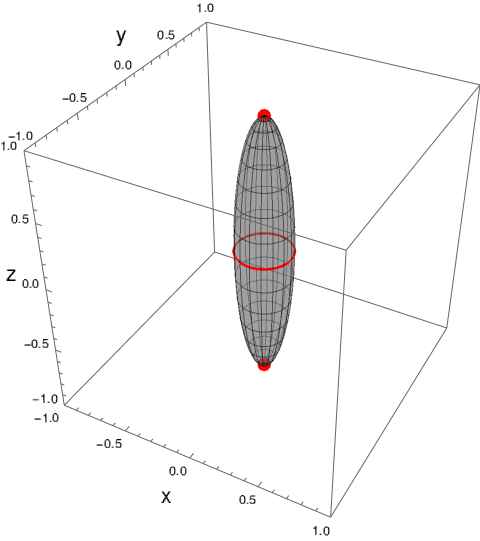
\includegraphics[width=0.6\linewidth]{chapter3/figures_toy/sphere_PF_t=1.0_z=0.8_p=0.6.png}
  \end{subfigure}
  \caption{Efecto de un canal de desfasamiento (no total) sobre la esfera de Bloch.}\label{fig:PhaseFlip}
\end{figure}
que reconocemos como un canal de desfasamiento total. Este resultado viene del hecho que, en el caso $p_{1}=1$, el estado de máxima entropía es simplemente $\rho_{\ef}\otimes\frac{\Id}{2}$. De manera similar, en el caso $p_{1}=0$, la dinámica efectiva es
\begin{equation}
  \Gamma_{t=1}(\rho_{\ef})=\frac{1}{2}\qty(\rho_{\ef}+\pauli{1}\rho_{\ef}\pauli{1}),\nonumber
\end{equation}
\begin{figure}[ht!]
  \centering
  \begin{subfigure}{0.5\textwidth}
    \centering
    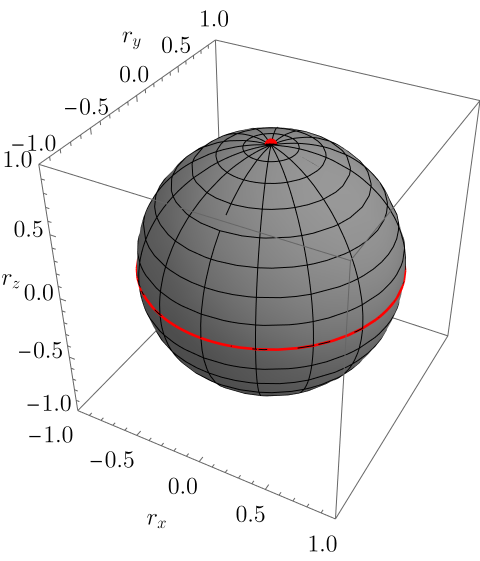
\includegraphics[width=0.6\linewidth]{chapter3/figures_toy/SWAP_t=0._p=0.9_r=0.9.png}
  \end{subfigure}%
  \begin{subfigure}{0.5\textwidth}
    \centering
    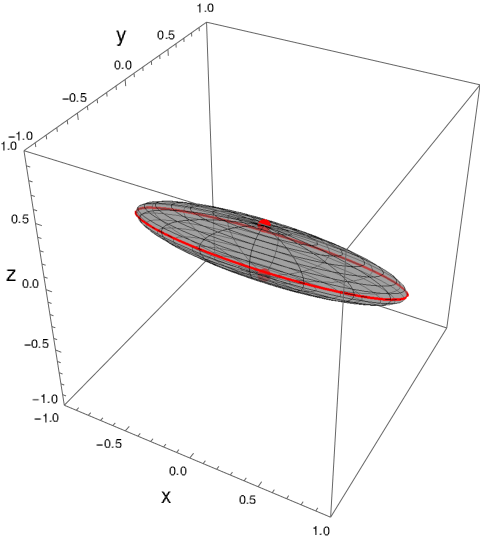
\includegraphics[width=0.6\linewidth]{chapter3/figures_toy/sphere_BitF_t=1.0_z=0.8_p=0.6.png}
  \end{subfigure}
  \caption{Efecto del canal de \textit{bit flip} (no completo) sobre la esfera de Bloch.}\label{fig:BitFlip}
\end{figure}
que no es más que un canal de \textit{bit flip} (que equivale a un canal de desfasamiento total si se trabaja en la base de los eigenestados de $\pauli{1}$). Sabiendo esto, es posible reacomodar la expresión de la dinámica efectiva para recuperar la transición entre estos casos extremos:
\begin{align}
  \Gamma_{t=1}(\rho_{\ef})=&\,\frac{1}{2}\rho_{\ef}\nonumber\\
  &+\frac{p_{1}}{2}\qty[\expval{\pauli{1}}_{\rho_{2}}\rho_{1}+(1-\expval{\pauli{1}}_{\rho_{2}})\pauli{3}\rho_{1}\pauli{3}]\nonumber\\
  &+\frac{p_{2}}{2}\qty[\expval{\pauli{3}}_{\rho_{1}}\rho_{2}+(1-\expval{\pauli{3}}_{\rho_{1}})\pauli{1}\rho_{2}\pauli{1}].\nonumber
\end{align}
De esta forma, el efecto de la dinámica efectiva es una combinación de dos canales no lineales: un canal de despolarización total en el que los coeficientes probabilísticos dependen del estado inicial, y un canal de \textit{bit flip} total con la misma característica. 

\subsubsection{CNOT efectivo a un tiempo arbitrario}

Estudiado el caso discreto, utilícese el hamiltoniano para propagar al estado microscópica de forma continua en el tiempo. El estado efectivo es propagado por la evolución efectiva
\begin{align}
  \Gamma_{t}(\rho_{\ef})=&\rho(\cos^{4}(\omega t)+\sin^{4}(\omega t))\nonumber\\
  &+p_{1}\{2\sin^{2}(\omega t)\cos^{2}(\omega
  t)\qty[\expval{\pauli{1}}_{2}\rho_{1}+\qty(1-\expval{\pauli{1}}_{\rho_{2}})\pauli{3}\rho_{1}\pauli{3}]\nonumber\\
  & \ \ \ \ \ \ \ +i(\sin^{3}(\omega t)\cos(\omega t)-\sin(\omega t)\cos^{3}(\omega t))\qty(1-\expval{\pauli{1}}_{\rho_{2}})[\rho_{1},\pauli{3}]\}\nonumber\\
  &+p_{2}\{2\sin^{2}(\omega t)\cos^{2}(\omega t)\qty[\expval{\pauli{3}}_{\rho_{1}}\rho_{2}+\qty(1-\expval{\pauli{3}}_{\rho_{1}})\pauli{1}\rho_{2}\pauli{1}]\nonumber\\
  &\ \ \ \ \ \ \ \ +i(\sin^{3}(\omega t)\cos(\omega t)-\sin(\omega t)\cos^{3}(\omega t))\qty(1-\expval{\pauli{3}}_{\rho_{1}})[\rho_{2},\pauli{1}]\}.\nonumber
\end{align} 
Esta expresión puede manipularse para recuperar algo más parecido a lo obtenido en el caso discreto,
\begin{align}\label{eq:EffectiveCNOT}
  \Gamma_{t}(\rho_{\ef})=&\frac{1}{2}\rho_{\ef}\nonumber\\
  &+\frac{p_{1}}{2}\{\rho_{1}\cos^{2}(2\omega t)+\qty[\expval{\pauli{1}}_{\rho_{2}}\rho_{1}+\qty(1-\expval{\pauli{1}}_{\rho_{2}})\pauli{3}\rho_{1}\pauli{3}]\sin^{2}(2\omega t)\nonumber\\
  & \ \ \ \ \ \ \ \ -i\qty(1-\expval{\pauli{1}}_{\rho_{2}})\cos(2\omega t)\sin(2\omega t)[\rho_{1},\pauli{3}]\}\nonumber\\
  &+\frac{p_{2}}{2}\{\rho_{2}\cos^{2}(2\omega t)+\qty[\expval{\pauli{3}}_{\rho_{1}}\rho_{2}+\qty(1-\expval{\pauli{3}}_{\rho_{1}})\pauli{1}\rho_{2}\pauli{3}]\sin^{2}(2\omega t)\nonumber\\
  & \ \ \ \ \ \ \ \ -i\qty(1-\expval{\pauli{3}}_{\rho_{1}})\cos(2\omega t)\sin(2\omega t)[\rho_{2},\pauli{1}]\}.
\end{align}
En esta ecuación ya se ve la acción de la evolución efectiva. El segundo y tercer términos pueden verse como canales de desfasamiento en dirección $\pauli{3}$ y $\pauli{1}$ respectivamente, pero contaminados con factores dependientes de los valores de expectación $\expval{\pauli{3}}_{\rho_{1}}$ y $\expval{\pauli{1}}_{\rho_{2}}$, que median la interacción entre las partículas. Para que esto sea aún más claro, volvamos a considerar los casos extremos de $p_{1}$.

Si $p_{1}=1$ entonces el estado de máxima entropía es $\rho_{\ef}\otimes\Id_{2}$, así que $\expval{\pauli{1}}_{\rho_{2}}=0$. La dinámica efectiva se reduce al canal de desfasamiento en dirección $\pauli{3}$
\begin{equation*}
  \Gamma_{t}(\rho_{\ef})=\frac{1}{2}\qty(\rho_{\ef}+e^{\rmi 2\omega t \pauli{3}}\rho_{\ef}e^{-\rmi 2\omega t \pauli{3}}).
\end{equation*}
Por otro lado, si $p_{1}=0$ el estado de máxima entropía es $\Id_{2}\otimes\rho_{\ef}$, así que $\expval{\pauli{3}}_{\rho_{1}}=0$ y la dinámica efectiva se reduce al canal de \textit{bit flip},
\begin{equation*}
  \Gamma_{t}(\rho_{\ef})=\frac{1}{2}\qty(\rho_{\ef}+e^{\rmi 2\omega t \pauli{1}}\rho_{\ef}e^{-\rmi 2\omega t \pauli{1}}).
\end{equation*}
En ambos casos recuperamos los resultados del caso discreto al tiempo $t=1$ eligiendo $\omega=\frac{\pi}{4}$. La dinámica generada por la compuerta CNOT es, nuevamente, una dinámica no solo no unitaria, sino no lineal, pues depende del estado efectivo inicial a través del multiplicador de Lagrange $\lambda$. La figura \ref{fig:AlmostBitFlipSequence} muestra la evolución para un valor de $p_{1}$ cercano a $0$, de tal forma que el término de \textit{bit flip} es dominante. La figura \ref{fig:AlmostPhaseFlipSequence}, en cambio, muestra la evolución para un valor de $p_{1}$ cercano a $1$ así que la evolución es casi un desfasamiento total. Finalmente, la figura \ref{fig:CNOTSequence} muestra la evolución para el caso $p_{1}=\frac{1}{2}$, en el que ninguno de los términos es dominante.
  \begin{figure}[ht!]
  \centering
  \begin{subfigure}{0.32\textwidth}
    \centering
    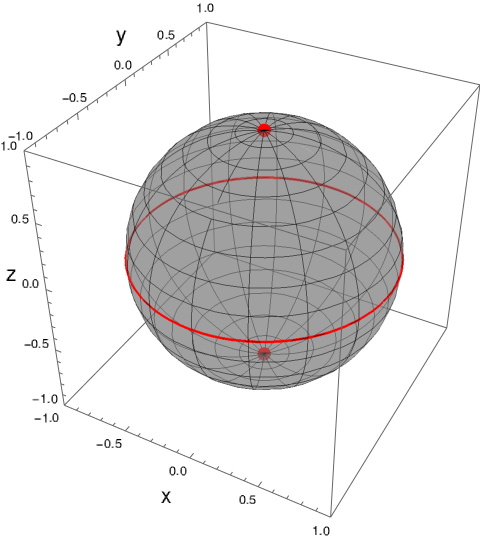
\includegraphics[width=0.9\linewidth]{chapter3/figures_toy/sphere_CNOT_t=0._r=0.9_p=0.1.png}
    \caption{$t=0$}
  \end{subfigure}%
  \begin{subfigure}{0.32\textwidth}
    \centering
    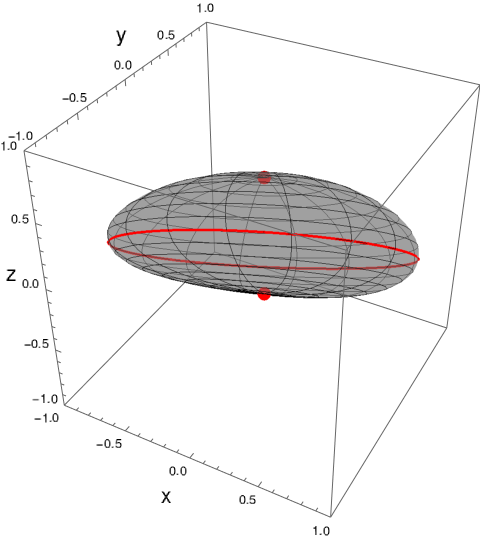
\includegraphics[width=0.9\linewidth]{chapter3/figures_toy/sphere_CNOT_t=0.5_r=0.9_p=0.1.png}
    \caption{$t=0.5$}
  \end{subfigure}
  \begin{subfigure}{0.32\textwidth}
    \centering
    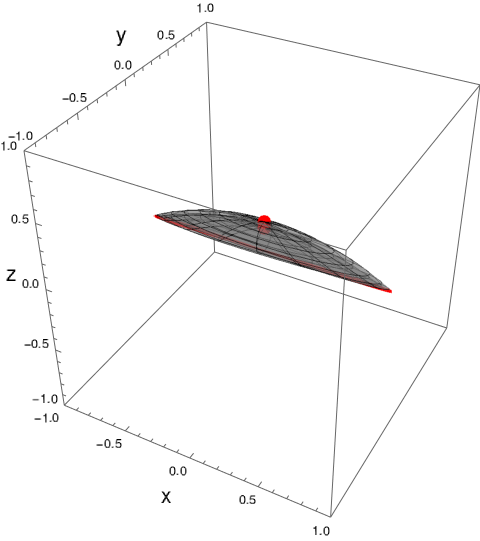
\includegraphics[width=0.9\linewidth]{chapter3/figures_toy/sphere_CNOT_t=1._r=0.9_p=0.1.png}
    \caption{$t=1$}
  \end{subfigure}
  \caption{Efecto de la evolución subyacente si $r_{z}=0.9$, $p=0.1$. Nótese que a tiempo $t=1$ se recupera el \textit{casi} canal de \textit{bit flip}. \ddnote{autocontenido}}
  \label{fig:AlmostBitFlipSequence}
  \end{figure}

  \begin{figure}[ht!]
    \centering
    \begin{subfigure}{0.32\textwidth}
      \centering
      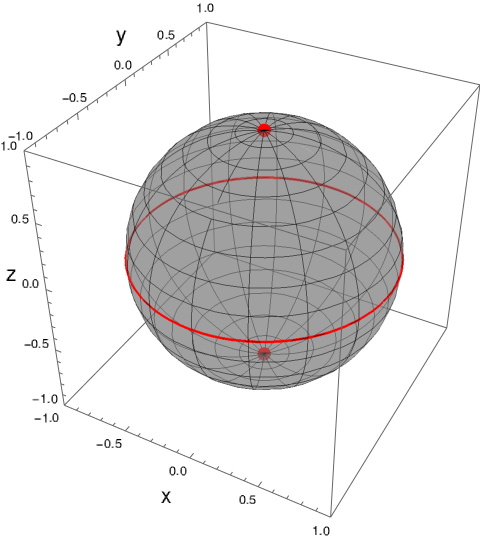
\includegraphics[width=0.9\linewidth]{chapter3/figures_toy/sphere_CNOT_t=0._r=0.9_p=0.1.png}
      \caption{$t=0$}
    \end{subfigure}%
    \begin{subfigure}{0.32\textwidth}
      \centering
      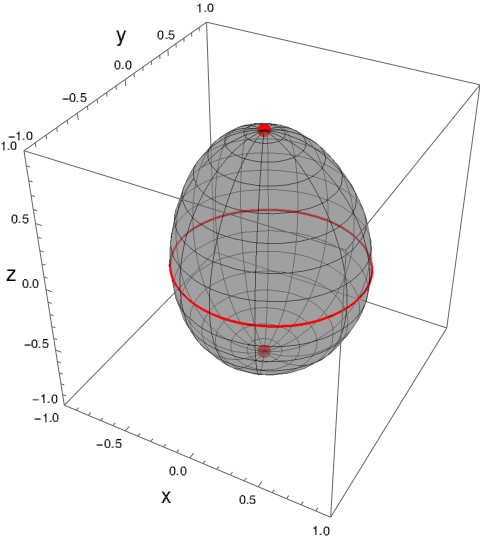
\includegraphics[width=0.9\linewidth]{chapter3/figures_toy/sphere_CNOT_t=0.5_r=0.9_p=0.9.png}
      \caption{$t=0.5$}
    \end{subfigure}
    \begin{subfigure}{0.32\textwidth}
      \centering
      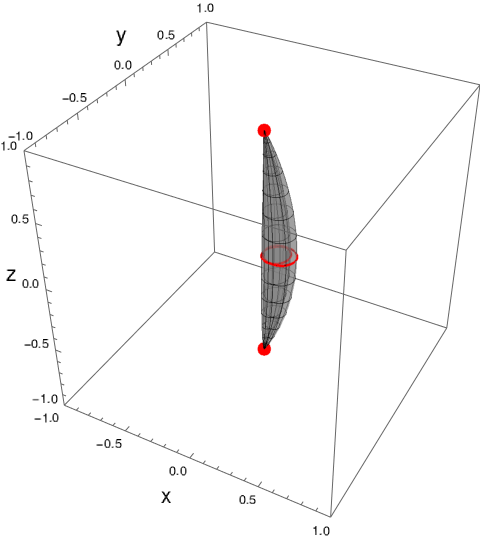
\includegraphics[width=0.9\linewidth]{chapter3/figures_toy/sphere_CNOT_t=1._r=0.9_p=0.9.png}
      \caption{$t=1$}
    \end{subfigure}
    \caption{Efecto de la evolución subyacente si $r_{z}=0.9$, $p=0.9$. Nótese que a tiempo $t=1$ se recupera el \textit{casi} canal de desfasamiento. \ddnote{autocontenido} }
    \label{fig:AlmostPhaseFlipSequence}
    \end{figure}

    \begin{figure}[ht!]
      \centering
      \begin{subfigure}{0.32\textwidth}
        \centering
        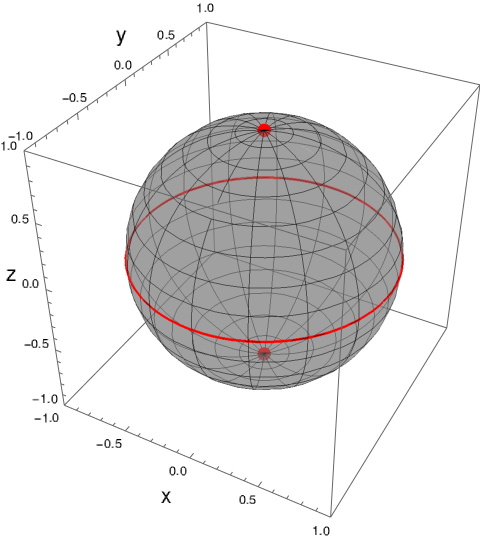
\includegraphics[width=0.9\linewidth]{chapter3/figures_toy/sphere_CNOT_t=0._r=0.9_p=0.1.png}
        \caption{$t=0$}
      \end{subfigure}%
      \begin{subfigure}{0.32\textwidth}
        \centering
        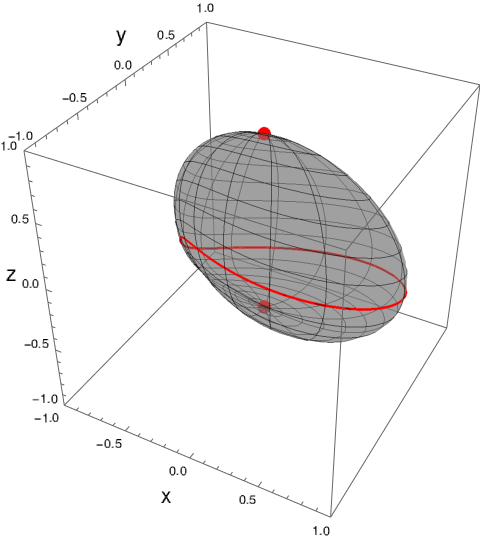
\includegraphics[width=0.9\linewidth]{chapter3/figures_toy/sphere_CNOT_t=0.5_r=0.9_p=0.5.png}
        \caption{$t=0.5$}
      \end{subfigure}
      \begin{subfigure}{0.32\textwidth}
        \centering
        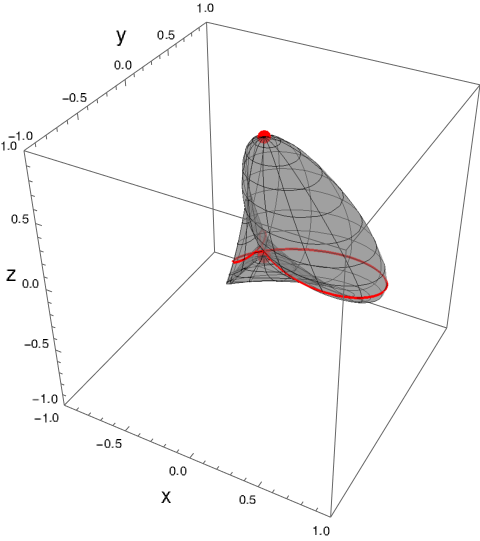
\includegraphics[width=0.9\linewidth]{chapter3/figures_toy/sphere_CNOT_t=1._r=0.9_p=0.5.png}
        \caption{$t=1$}
      \end{subfigure}
      \caption{Efecto de la evolución subyacente si $r_{z}=0.9$, $p=0.5$. La deformación (y rompimiento) de la esfera de Bloch es consecuencia de la combinación de dos canales no lineales. \ddnote{autocontenido}}
      \label{fig:CNOTSequence}
      \end{figure}
      \newpage




      